%!TEX root = ../template.tex
%%%%%%%%%%%%%%%%%%%%%%%%%%%%%%%%%%%%%%%%%%%%%%%%%%%%%%%%%%%%%%%%%%%
%% chapter1.tex
%% NOVA thesis document file
%%
%% Chapter with introduction
%%%%%%%%%%%%%%%%%%%%%%%%%%%%%%%%%%%%%%%%%%%%%%%%%%%%%%%%%%%%%%%%%%%

\typeout{NT FILE chapter1.tex}%

\chapter{Introduction}
\label{cha:introduction}

\prependtographicspath{{Chapters/Figures/Introduction}}

%% Plan:

% Introduction

% - Vagus Nerve Stimulation

% - Technological Context

%   - CMOS Scaling

%   - Embedded Feature Extraction

% - Problem Definition

% - Research Question


\section{Motivation}
\label{sec:motivation}

\subsection{World Health: Current context}
\label{subsec:world_health_context}

\begin{figure}[bp]
    \centering
    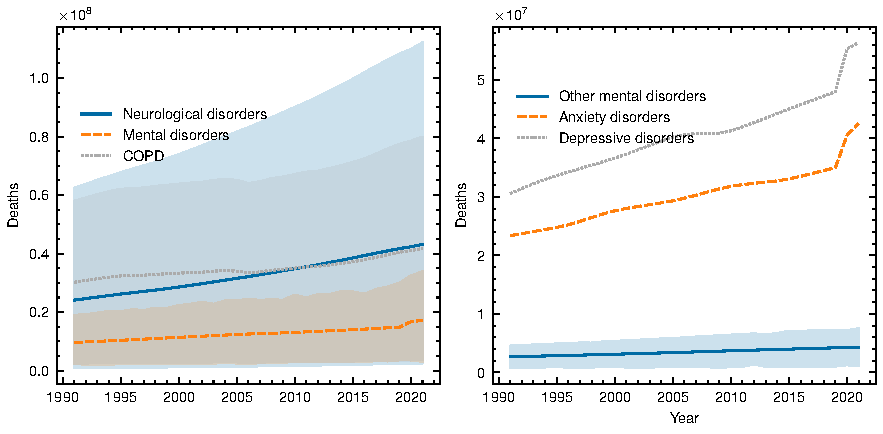
\includegraphics[width=1.0\textwidth]{Chapters/Figures/Introduction/deaths_neuro_mental_disorders.pdf}
    \caption{a) Yearly number of deaths associated to neurological, mental and chronic obstructive pulmonary diseases (COPD), according to the WHO, b) Discrimination of number of deaths associated to depressive and anxiety disorders relative to other mental disorders. Data retrieved from \cite{https://ghdx.healthdata.org/record/ihme-data/gbd-2021-nervous-system-disorders-1990-2021}}
    \label{fig:deaths_mental_disorders}
\end{figure}

\par
The leading cause of illness and disability worldwide are neurological disorders, affecting approximately a third of the world's population \cite{WorldHealthOrg}. Such disabilities can have a profound impact on memory, cognition, personality, movement, and essential physiological mechanisms such as breeding \cite{}. The global trend on the occurrence of neurological disorders such as depression, epileptic seizures and Parkinson's disease has been toward a rapid increase, prevailing, in relevance, alongside other current health epidemics such as cancer and cardiovascular disorders \cite{}. In light of the current world health context, the development of new clinical therapeutic and diagnostic interventions is of utmost importance, allowing safer, more comfortable, and highly effective alternatives to existing medical procedures.

\par
Pharmaceuticals remain the traditional approach to the treatment of diseases.
However, it is well established that the use of commercially available synthesized drugs affects the whole body, often inducing side effects that can lead to a decrease in patient quality of life\cite{Goggins2022, Ji2020}. 
Moreover, recent pharmacoeconomic studies suggest that the research and 
development of new Pharmaceuticals costs range from \$161 million and \$4.54 billion, with additional costs of introducing new drugs into the market achieving \$880 million \cite{https://www.nature.com/articles/d41573-024-00130-3, 10.1007/s40273-021-01065-y}. 
The complexity of the nervous system renders the aforementioned costs to be 
significantly optimistic \cite{}. The development of drugs capable of tackling 
neurological diseases efficiently is limited by the available drug delivery methods, 
especially when delivering pharmaceuticals directly to the brain \cite{}. The semipermeable 
blood-brain barrier regulates the transfer of chemical compounds between the 
circulatory and nervous system, rendering existing pharmaceutical drugs quite 
ineffective. Developing targeted drug delivery systems requires a parallel investment 
in research and development that can achieve similar investment magnitudes to 
the ones redirected towards drug development \cite{}. This increase in spending 
has not produced positive results. While the global spending in new pharmaceutical drugs' research and development (R\&D) has featured an increasing trend for the past 30 years, the same rising trend can be observed in the casualties associated to neurological, mental and chronic obstructive pulmonary disorders (COPD) (Fig. \ref{fig:motivation_who_records}) - suffering a drastic increase during and post-COVID-19 years.

\begin{figure}[bh]
    \centering
    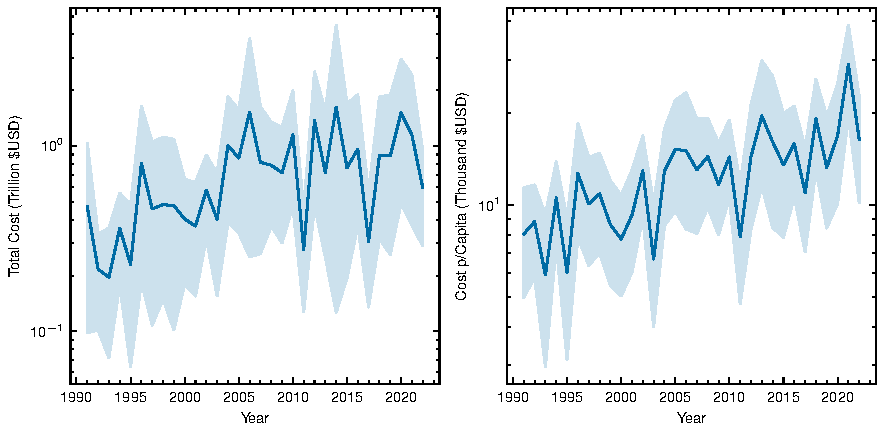
\includegraphics[width=1.0\textwidth]{Chapters/Figures/Introduction/r_and_d_spending.pdf}
    \caption{Yearly global pharmaceutical 
  drug R\&D spending in US Dollars (\$USD) a) in total b) per capita  \cite{https://github.com/datasets/pharmaceutical-drug-spending}.}
    \label{fig:r_and_d_spending_worldwide}
\end{figure}

\par
The total health-care spending is only projected to grow, leading scientists to believe that pharmaceutical drug R\&D has been, so far, quite ineffective in the task of tackling diseases directly linked to the nervous system \cite{}. While prevention will always be the most affordable and effective method to tackle most diseases, the genetic nature most neurological medical conditions feature remains a challenge that has been most effectively tackled by non-pharmaceutical treatments directly targeting the nervous system of each clinical subject \cite{}.

\subsection{Vagus Nerve: A window of opportunity}
\label{subsec:vagus_nerve}

\par
The vagus nerve (VN) is the longest cranial nerve in the human body, extending
from the brainstem to the abdomen through multiple organs such as the heart,
lungs, stomach and intestines. The VN is responsible for the regulation of the
parasympathetic nervous system (PNS). Due to its central role on the function of the
PNS, multiple studies have shown that the VN can be stimulated to offer therapeutic
procedures to conditions such as blood-pressure (BP) regulation, epileptic seizure
suppression, mood and apetite control and chronic pulmonary obstructive disease
(COPD) \cite[*]{Goggins2022, Ji2020, Lescrauwaet2022, Browning2017, Undem2005}. 
Regarding mood control, vagus nerve stimulation (VNS) has also been shown as a potent intervention to tackle depression, once it offers targetted therapeutic methods modulating the PNS \cite{DepressionVNS}. Epileptic seizure suppression \cite{} and depression and mood control \cite{}, are examples of clinically approved VNS therapeutic procedures that have already underwent clinical trials, and are currently making an impact on the lives of the respective patients. Currently undergoing pre-clinical and clinical trials are the therapeutic applications of blood pressure regulation, appetite control for tackling the obesity epidemic \cite{},  chronic obstructive pulmonary disease \cite{} and Chron's disease \cite{}. 

\par
Neuromodulation-based therapeutic treatments have emerged as a promising method 
for tackling neurological disorders. Stimulation and suppression of neurological circuits by, respectively, activating or inhibiting neuronal activity enable the modulation of physiological and neurological functions \cite{Fomenko2018,Dalecki2004}. Several modalities of clinical procedures exist to perform VNS. 

\begin{figure}[ht]
  \centering
  \includegraphics[width=\textwidth]{Chapters/Figures/implantableVNS.png}
  \label{fig:implantable_electrode_vns}
\end{figure}

\it{Implantable VNS (iVNS)} requires electrodes directly implanted into the VN, enabling its precise stimulation up to individual nerve fibers. However, this invasive method requires a surgical procedure to subcutaneously implant the electrical stimulation system and an electrode cuff wrapped around the VN near carothid artery (CA) and jugular vein (JV) in the neck region of the patient \cite{}. The required surgical procedures introduces several unnecessary risks that also affect the time required to integrate implantable VNS applications in the market due to the required FDA approval \cite{}. 

\begin{figure}[ht]
  \centering
  \includegraphics[width=\textwidth]{Chapters/Figures/transcutaneousAuricularVNS.png}
  \label{fig:transcutaneous_electrode_vns}
\end{figure}

\it{Transcutaneous VNS (tVNS)} involves the stimulation of the VN using electrical currents induced by surface electrodes placed in direct contact with the skin of the patient \cite{}. This non-invasive method of VNS usually targets the auricular and cervical branches of the VN, and requires an auricular device containing an electrode to induce the electrical currents in a skin surface that is close enough to the target nerve \cite{}.
While being less invasive, this method is incapable of achieving high-precision stimulation through the stimulation of specific regions of the VN. This limited spatial precision renders the VNS procedures to be very limited regarding the possible therapeutic outcomes and applications of this method \cite{}.

\begin{figure}[ht]
  \centering
  \includegraphics[width=\textwidth]{Chapters/Figures/target_fUSVNS.png}
  \label{fig:fus_vns}
\end{figure}

Due to its location is closer to the skin surface, targeting the VN through
the human neck using low-intensity focused ultrasound (LIFUS) enables safer and
effective non-invasive methods to perform VNS \cite{Fomenko2018, Rivandi2023, Costa2021, Costa2019}.
\it{Ultrasound-based VN neuronomodulation (fUS-VNS)} has emerged as a promising method to enable spatially precise VNS procedures targetting a wide range of applications. 
Moderately increasing the fundamental, central frequency of the US focused beam 
enables a high lateral precision when delivering a significant amount of energy to the 
arbitrary VN region thorugh the fUS focal spot \cite{}.

Moreover, existing studies on the impact of VNS on the nervous system of mammals are currently limited by the clinical apparatus required to conduct and measure the impact of VNS on the test subjects, especially when they're aimed at macaques or/and humans. The need for implantable VNS medical devices greatly increases the time it takes to obtain FDA approval to conduct such studies. The limited applicability of tVNS on the range of possible therapeutical applications makes fUS-VNS specially promising for next generation exploratory clinical devices \cite{}. The ability to integrate both reliable imaging and stimulation systems in the same ASIC has become a much wanted goal and and has sprouted an active research field on integrated US medical devices - not only for its implications on the future of point-of-care (POC) therapeutic devices for neurological disorders, but also for mitigating the procedural complexity of using fUS apparatus to target the VN upon conducting exploratory clinical procedures, as discussed in more detail in the next section \cite{}.

\section{Clinical Ultrasound Practice}
\label{sec:clinical_ultrasound_practice}

\subsection{Ultrasound Neuromodulation Mechanisms}
\label{subsec:ultrasound_neuromodulation_mechanisms}

\subsection{Ultrasound in the Clinic}
\label{subsec:ultrasound_in_the_clinic}



\section{Challenges in Ultrasound Image-Guided Neuromodulation Integrated Systems}
\label{sec:problem_definition}

\subsection{Effective Vagus Nerve Stimulation}
\label{subsec:effective_vagus_nerve_stimulation}

The efficiency of therapeutic procedures associated with VNS is guaranteed by
ensuring that the sonication protocol is properly applied and US beam energy transfer 
to the target is optimized. The required lower US centre sonication frequency to achieve lower US signal attenuation when trying to perform non-invasive US imaging
(and stimulation) of the vagus nerve through the human neck's muscle
wall conditions the reconstructed US 2D US \textit{brightness-mode} (B-mode) image to low spatial resolution \cite{Szabo2014_1_8_2_Ultrasound}. Probe placement mismatch and the risk of US image mis-interpretation increases the influence of human-error when
targetting the VN through the application of the control-loop
presented in Fig. \ref{fig:vagus_nerve_stim_apps} e). Additionally, 
the vagus nerve can present six different positions according to reported 
anatomical studies, further increasing the difficulty of identifying the correct 
patient-specific location of the vagus nerve in real time, 
even for trained physicians \cite{}.

Finally, when targetting the VN while varying the US sonication protocol
parameters to explore the influence of each parameter on the
patient's response to the VNS procedure, the VN's location must be
accurately recognized and targeted to ensure an higher confidence
level on the results of the therapeutic procedure. Failing to target
the VN leads to an ineffective clinical therapeutic or scientific
exploration session \cite{Ahmed2022}.
\par

%A growing interest in the
%development of automated systems performing the recognition of the
%VN's location in the US B-mode image, aiding trained physicians by reducing 
%human-induced error possibility \cite{Drukker2020, Young2021, Huan2024}.
%\textit{Machine learning} (ML) algorithms enable real-time
%recognition of the vagus nerve location  in the US B-mode image by
%constraining the time overhead of the algorithm to the training
%process of the ML model. The extracted position or region of interest
%(ROI) of the VN in the US B-mode can then be used to guide the LIFUS
%wave to the target location, ensuring the effectiveness of the VNS
%procedure \cite{Drukker2020, Battal2021}. However, current efforts
%optimize feature extraction processes using
%high-level alogrithms running on general purpose complex processing 
%units such as the \textit{central processing unit} (CPU) or the
%\textit{graphics processing unit} (GPU). Template-image based algorithm 
%have also been recently proposed to reduce the hardware complexity required 
%to perform VN location detection, but it still requires the use of a dedicated 
%digitally-heavy processing unit implemented using an field-programmable gate array %(FPGA) 
%placed at the back end of the signal acquisition chain \cite{Huan2024}.
%As such, current research efforts US
%scatterer localization are based on low-portability and/or power-hungry
%solutions placed at the back end of the signal acquisition chain
%\cite{Battal2021, ChangKyo2021, Youn2020, Nair2020}.

\subsection{Ultrasound Imaging ASIC Output Data-Rate and Power Dissipation Requirements}
\label{subsec:ultrasound_imaging_data_rate}
In general, two main methods of performing US imaging 
exist: 1) planar wave compounding (PWC) imaging and 2) scan-line (SL) imaging \cite{Szabo2014}. SL imaging enables golden-standard US imaging quality, once ultrasound is two-way focused -- an US beamline is focused on a point in a numerically predefined imaging grid using a convex lens. Because the recovered echoes from that focused point in space are assumed to carry the majority of the power (assuming negligible secondary lobe energy), an inverse concave lens can be directly used to reconstruct the spatial information of the medium from the temporal information received. Contrarily, planar wave imaging methods such as PWC do not focus US in a single beam profile, but rather introduce controlled phase delays in the transmitted pulses to create a planar wavefront sonicating the whole imaging media at once. As such, during reception, the information of the medium arrives highly correlated between each point of the imaging grid, and must be recovered simultaneously before starting the reconstruction of the US image. Both methods require high data-rates to transmit the high volume of samples generated by the US transducer array to the back-end data processing unit. Digital communication of the quantized information greatly increases the US imaging ASIC's output signal integrity. 
However, the high data-rate requirements lead to high power dissipation on the quantizer stages, the biasing circuitry, high-speed serial communication
interfaces and ASIC output load drivers \cite{Hopf2023, Chen2017, 
Tan2018, Jung2018}. 

\begin{figure}[bp]
  \centering
  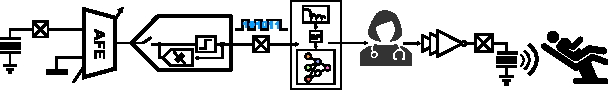
\includegraphics[width=\textwidth]{Chapters/Figures/Introduction/high_power_approach.pdf}
  \label{fig:high_power_solution}
  \caption{An envisaged US imaging ASIC in a typical fUS therapeutic clinical procedure  information flux. An ultrasound image can be reconstructed from the recovered echoes, transported to the image reconstruction and data acquisition system in digital domain for higher signal integrity reliability.}
\end{figure}


\begin{equation}
  P_{SER} = p_1 \ F_S \ C_{Line} V_{DDD}^2 \ = 0.66 \cdot 50\mathrm{MHz} \cdot 4\mathrm{pF} \cdot {(0.9\mathrm{V})}^2 = 27\mathrm{mW}
  \label{eq:serial_power_dissipation}
\end{equation}

As an example, let us consider an US imagig ASIC integrated within a PCB with a digital processing backend (Fig) performing an image acquisition. Depending on the metal trace width and length, the PCB connection between both chips can easily achieve a 1 - 4pF parasitic capacitance ($C_{Line}$). The system features 32 channels, with an 8 bit quantizer per stage, operating at a nominal sampling frequency ($F_S$) of 50 MHz. The total bit rate achieves $32 \cdot 8b \cdot 50 \ \mathrm{MHz} = 1.6 \ \mathrm{Gbyte/s}$. Considering that the US imaging ASIC's serial communication line, biased at a digital supply ($V_{DDD}$) of 0.9V, presents a 66\% chance ($p_1$) of transmitting a logic "1", then the total dynamic power dissipation of the serial transmission ($P_{SER}$) can easily achieve 27mW, as observed from (\ref{eq:serial_power_dissipation}). If we consider that each AFE channel features a total power dissipation of 1.0mW, a value well within the state of the art, then the total power dissipation of the 32 channels is 32mW. Almost the same amount of power is dissipated in acquiring and processing the echo signals as well as exporting them out of the ASIC due to the very high data throughput required when performing US imaging. Moreover, this problem is aggravated when interfacing thousands of channels. A typical state-of-the-art US imaging system interfaces with a transducer matrix capable of 3D imaging by stacking multiple 2D B-mode image slices together, and to achieve enough resolution to enable the distinction of the complex anatomy of the human neck, at least 32-by-32 (1024) channels are required. 

\section{Dissertation Goal and Thesis Plan Organization}
\label{subsec:goal_and_organization}

%TODO: introduce citations

Both preclinical and clinical studies can become great benefactors of miniaturized US transducer arrays that allow for targetting different regions of the VN, at different intensities and levels of spatial precision, once the variation of these parameters can lead to new insights and unlock new treatments. However, the targeting of the VN is a complex procedure that must be guaranteed to provide enough confidence level in the obtained results of the exploratory procedure, as well as guaranteeing the safety of future users of an envisaged wearable fUS VNS device. As discussed above, the guidance of the focused beam has been performed using bulky medical imaging devices, introducing a significant level of procedural and bureaucratic complexity that can lead to the cost increase of each study as well, as decreasing the celerity of the its conclusion. An integrated, minimally invasive, reconfigurable, wearable device capable of reliable US imaging as well as fUS stimulation has the potential remove these barriers.

\par
The pursuit for the miniaturization of US imaging-enabled ASICs has led most research groups to tackle the problem of power dissipation reduction from an IC-design perspective solemnly. However, as further addressed, the decisions on how the integration between the sensor matrix and the interfacing integrated electronics are performed have the possibility of drastically impacting both the power dissipation of the data readout system as well as mechanically compressing the information on the phase of the received US echoes. Further compression can also be achieved by adopting a channel multiplexing strategy that effectively preserves the phase information of the received echoes, enabling an higher signal-to-noise (SNR) ratio in the reconstructed images. Moreover, these sensor integration decisions, combined with possible system-design choices, also allow vast amounts of free and additional space inside an IC that can be used to introduce a more complex, and refined control of power-efficient high-voltage (HV) pulsers to finally converge towards a wearable device capable of US imaging and stimulation that complies with FDA regulations regarding the safety of the device upon its direct interface with the patient. The focus of these work is the development of an highly miniaturized, and energy efficient US imaging device, capable of seamless integration within a low-form-factor wearable system with the ability of FUS beam-steering for VNS (Fig. \ref{fig:main_goal}). 

\par
A brief, but necessary introduction to US waves and their physical properties, the transducers used to perform a bidirectional translation of US into electrical signals, and US imaging algorithms and system specifications is discussed in Chapter \ref{cha:ultrasound_transducers_and_ultrasound_imaging}.  
Insightful discussions on the current methods used to address the power dissipation limitations and the data throughput of an US imaging system are provided in Chapter \ref{cha:state-of-art}.  These discussions include a) which ultrasound transducer materials are best suited for each US application, with a special focus on the most suitable materials and transducer architectures for a FUS stimulation application and its implications regarding the image quality of these transducers, b) currently existing transducer matrix-interfacing electronics integration methods and their implications towards the quality and resolution of the reconstructed US images and c) state-of-the-art ASICs for US echoes readout, with a special focus on the methods used to compress the number of output channels of the US RX system and the associated channel multiplexing schemes, promoting the power dissipation and output data-throughput reduction of the system. The implication of these channel multiplexing schemes on the compression of the sampled US echoes in the axis of time is also discussed, at it is of utmost importance to infer on the required number of discrete-time US echo samples required to reconstruct a reliable US image. Chapter \ref{cha:state_of_the_art} culminates in the research questions selected to be addressed in this dissertation. Finally, Chapter \ref{cha:literature_review_methodology_and_workplan} provides a description of the methods used to select the scientific peer-reviewed material, and its sources, used to establish the ideas discussed throughout this dissertation plan, ending with a presentation of the devised  work plan to be developed to achieve the goal of this dissertation.



%Instead of retrieving all the required data to reconstruct an ultrasound image, 
%so that the position of the VN can be detected, another possible solution would be to 
%perform the detection of the VN directly on chip using an analog inference system.

%\subsection{Towards On-Chip Feature Extraction in Ultrasound Image-Guided Stimulation}
%\label{subsec:on_chip_feature_extraction}
%
%Conventional biomedical application system architectures are
%constituted by a front-end signal acquisition interface and a
%back-end data processing unit to perform feature extraction. The high
%amount of data generated by the front-end signal acquisition
%interface requires high data-rates to be sent to the back-end data
%processing unit, leading to high power-dissipation. The integration
%of feature extraction algorithms closer to the sensor enables this operation 
%to be performed with a lower time-overhead and
%power-dissipation, once only the extracted features are trasnmitted
%\cite{vanAssche2023}. On-chip feature extraction has observed a growing trend,
% shown to eliminate the need for the use of GPUs and CPUs on the back-end of the application
%\cite{Azghadi2020, vanAssche2023}. Moreover, recent ML accelerator architecture research 
%trends show that analog-based integrated circuits enable 
%optimal power-dissipation when implementing feature extraction, regression and 
%classification algorithms while maintaining similar computational 
%speed compared to their digital counterpart \cite{Tsai2018, Haensch2019, Xiao2020}. 
%
%Integrating the ML system closer to the sensor
%could enhance cost effectiveness, power-efficiency, accessibility and
%commodity for patients and medical professionals by increasing the
%portability of the medical imaging apparatus, effectively enabling
%true point-of-care (POC) applications \cite{vanAssche2023, Damak2021}.

%\subsection{Proposed Solution}
%\label{subsec:proposed_solution}

%The objective of this dissertation is to converge towards an US RX system that is capable of 
%acquiring the ultrasound signals using a dedicated analog-front end (AFE) aiming to minimize the 
%total dissipated power, as well as detecting the VN position using an on-chip regression 
%analog neural network (ANN). The block-diagram of the system is represented in Fig. \ref{fig:block_diagram}. 
%The target system integrates a multiplexed imaging path and analog inference path. When the 
%inference path is selected, the regression ANN performs the detection of the VN position from the 
%US RF time-series data directly. On the other hand, to guarantee the safety of patient when subjected 
%the application, and to mitigate the impact of the regression error, the imaging path can be selected 
%to enable the reconstruction of an US B-mode image to allow for the observation of the sonicated medium, 
%and for the recalibration of the ANN.